% Options for packages loaded elsewhere
\PassOptionsToPackage{unicode}{hyperref}
\PassOptionsToPackage{hyphens}{url}
\PassOptionsToPackage{dvipsnames,svgnames,x11names}{xcolor}
%
\documentclass[
  letterpaper,
  DIV=11,
  numbers=noendperiod]{scrreprt}

\usepackage{amsmath,amssymb}
\usepackage{iftex}
\ifPDFTeX
  \usepackage[T1]{fontenc}
  \usepackage[utf8]{inputenc}
  \usepackage{textcomp} % provide euro and other symbols
\else % if luatex or xetex
  \usepackage{unicode-math}
  \defaultfontfeatures{Scale=MatchLowercase}
  \defaultfontfeatures[\rmfamily]{Ligatures=TeX,Scale=1}
\fi
\usepackage{lmodern}
\ifPDFTeX\else  
    % xetex/luatex font selection
\fi
% Use upquote if available, for straight quotes in verbatim environments
\IfFileExists{upquote.sty}{\usepackage{upquote}}{}
\IfFileExists{microtype.sty}{% use microtype if available
  \usepackage[]{microtype}
  \UseMicrotypeSet[protrusion]{basicmath} % disable protrusion for tt fonts
}{}
\makeatletter
\@ifundefined{KOMAClassName}{% if non-KOMA class
  \IfFileExists{parskip.sty}{%
    \usepackage{parskip}
  }{% else
    \setlength{\parindent}{0pt}
    \setlength{\parskip}{6pt plus 2pt minus 1pt}}
}{% if KOMA class
  \KOMAoptions{parskip=half}}
\makeatother
\usepackage{xcolor}
\setlength{\emergencystretch}{3em} % prevent overfull lines
\setcounter{secnumdepth}{5}
% Make \paragraph and \subparagraph free-standing
\makeatletter
\ifx\paragraph\undefined\else
  \let\oldparagraph\paragraph
  \renewcommand{\paragraph}{
    \@ifstar
      \xxxParagraphStar
      \xxxParagraphNoStar
  }
  \newcommand{\xxxParagraphStar}[1]{\oldparagraph*{#1}\mbox{}}
  \newcommand{\xxxParagraphNoStar}[1]{\oldparagraph{#1}\mbox{}}
\fi
\ifx\subparagraph\undefined\else
  \let\oldsubparagraph\subparagraph
  \renewcommand{\subparagraph}{
    \@ifstar
      \xxxSubParagraphStar
      \xxxSubParagraphNoStar
  }
  \newcommand{\xxxSubParagraphStar}[1]{\oldsubparagraph*{#1}\mbox{}}
  \newcommand{\xxxSubParagraphNoStar}[1]{\oldsubparagraph{#1}\mbox{}}
\fi
\makeatother

\usepackage{color}
\usepackage{fancyvrb}
\newcommand{\VerbBar}{|}
\newcommand{\VERB}{\Verb[commandchars=\\\{\}]}
\DefineVerbatimEnvironment{Highlighting}{Verbatim}{commandchars=\\\{\}}
% Add ',fontsize=\small' for more characters per line
\usepackage{framed}
\definecolor{shadecolor}{RGB}{241,243,245}
\newenvironment{Shaded}{\begin{snugshade}}{\end{snugshade}}
\newcommand{\AlertTok}[1]{\textcolor[rgb]{0.68,0.00,0.00}{#1}}
\newcommand{\AnnotationTok}[1]{\textcolor[rgb]{0.37,0.37,0.37}{#1}}
\newcommand{\AttributeTok}[1]{\textcolor[rgb]{0.40,0.45,0.13}{#1}}
\newcommand{\BaseNTok}[1]{\textcolor[rgb]{0.68,0.00,0.00}{#1}}
\newcommand{\BuiltInTok}[1]{\textcolor[rgb]{0.00,0.23,0.31}{#1}}
\newcommand{\CharTok}[1]{\textcolor[rgb]{0.13,0.47,0.30}{#1}}
\newcommand{\CommentTok}[1]{\textcolor[rgb]{0.37,0.37,0.37}{#1}}
\newcommand{\CommentVarTok}[1]{\textcolor[rgb]{0.37,0.37,0.37}{\textit{#1}}}
\newcommand{\ConstantTok}[1]{\textcolor[rgb]{0.56,0.35,0.01}{#1}}
\newcommand{\ControlFlowTok}[1]{\textcolor[rgb]{0.00,0.23,0.31}{\textbf{#1}}}
\newcommand{\DataTypeTok}[1]{\textcolor[rgb]{0.68,0.00,0.00}{#1}}
\newcommand{\DecValTok}[1]{\textcolor[rgb]{0.68,0.00,0.00}{#1}}
\newcommand{\DocumentationTok}[1]{\textcolor[rgb]{0.37,0.37,0.37}{\textit{#1}}}
\newcommand{\ErrorTok}[1]{\textcolor[rgb]{0.68,0.00,0.00}{#1}}
\newcommand{\ExtensionTok}[1]{\textcolor[rgb]{0.00,0.23,0.31}{#1}}
\newcommand{\FloatTok}[1]{\textcolor[rgb]{0.68,0.00,0.00}{#1}}
\newcommand{\FunctionTok}[1]{\textcolor[rgb]{0.28,0.35,0.67}{#1}}
\newcommand{\ImportTok}[1]{\textcolor[rgb]{0.00,0.46,0.62}{#1}}
\newcommand{\InformationTok}[1]{\textcolor[rgb]{0.37,0.37,0.37}{#1}}
\newcommand{\KeywordTok}[1]{\textcolor[rgb]{0.00,0.23,0.31}{\textbf{#1}}}
\newcommand{\NormalTok}[1]{\textcolor[rgb]{0.00,0.23,0.31}{#1}}
\newcommand{\OperatorTok}[1]{\textcolor[rgb]{0.37,0.37,0.37}{#1}}
\newcommand{\OtherTok}[1]{\textcolor[rgb]{0.00,0.23,0.31}{#1}}
\newcommand{\PreprocessorTok}[1]{\textcolor[rgb]{0.68,0.00,0.00}{#1}}
\newcommand{\RegionMarkerTok}[1]{\textcolor[rgb]{0.00,0.23,0.31}{#1}}
\newcommand{\SpecialCharTok}[1]{\textcolor[rgb]{0.37,0.37,0.37}{#1}}
\newcommand{\SpecialStringTok}[1]{\textcolor[rgb]{0.13,0.47,0.30}{#1}}
\newcommand{\StringTok}[1]{\textcolor[rgb]{0.13,0.47,0.30}{#1}}
\newcommand{\VariableTok}[1]{\textcolor[rgb]{0.07,0.07,0.07}{#1}}
\newcommand{\VerbatimStringTok}[1]{\textcolor[rgb]{0.13,0.47,0.30}{#1}}
\newcommand{\WarningTok}[1]{\textcolor[rgb]{0.37,0.37,0.37}{\textit{#1}}}

\providecommand{\tightlist}{%
  \setlength{\itemsep}{0pt}\setlength{\parskip}{0pt}}\usepackage{longtable,booktabs,array}
\usepackage{calc} % for calculating minipage widths
% Correct order of tables after \paragraph or \subparagraph
\usepackage{etoolbox}
\makeatletter
\patchcmd\longtable{\par}{\if@noskipsec\mbox{}\fi\par}{}{}
\makeatother
% Allow footnotes in longtable head/foot
\IfFileExists{footnotehyper.sty}{\usepackage{footnotehyper}}{\usepackage{footnote}}
\makesavenoteenv{longtable}
\usepackage{graphicx}
\makeatletter
\def\maxwidth{\ifdim\Gin@nat@width>\linewidth\linewidth\else\Gin@nat@width\fi}
\def\maxheight{\ifdim\Gin@nat@height>\textheight\textheight\else\Gin@nat@height\fi}
\makeatother
% Scale images if necessary, so that they will not overflow the page
% margins by default, and it is still possible to overwrite the defaults
% using explicit options in \includegraphics[width, height, ...]{}
\setkeys{Gin}{width=\maxwidth,height=\maxheight,keepaspectratio}
% Set default figure placement to htbp
\makeatletter
\def\fps@figure{htbp}
\makeatother

\KOMAoption{captions}{tableheading}
\makeatletter
\@ifpackageloaded{bookmark}{}{\usepackage{bookmark}}
\makeatother
\makeatletter
\@ifpackageloaded{caption}{}{\usepackage{caption}}
\AtBeginDocument{%
\ifdefined\contentsname
  \renewcommand*\contentsname{Table of contents}
\else
  \newcommand\contentsname{Table of contents}
\fi
\ifdefined\listfigurename
  \renewcommand*\listfigurename{List of Figures}
\else
  \newcommand\listfigurename{List of Figures}
\fi
\ifdefined\listtablename
  \renewcommand*\listtablename{List of Tables}
\else
  \newcommand\listtablename{List of Tables}
\fi
\ifdefined\figurename
  \renewcommand*\figurename{Figure}
\else
  \newcommand\figurename{Figure}
\fi
\ifdefined\tablename
  \renewcommand*\tablename{Table}
\else
  \newcommand\tablename{Table}
\fi
}
\@ifpackageloaded{float}{}{\usepackage{float}}
\floatstyle{ruled}
\@ifundefined{c@chapter}{\newfloat{codelisting}{h}{lop}}{\newfloat{codelisting}{h}{lop}[chapter]}
\floatname{codelisting}{Listing}
\newcommand*\listoflistings{\listof{codelisting}{List of Listings}}
\makeatother
\makeatletter
\makeatother
\makeatletter
\@ifpackageloaded{caption}{}{\usepackage{caption}}
\@ifpackageloaded{subcaption}{}{\usepackage{subcaption}}
\makeatother

\ifLuaTeX
  \usepackage{selnolig}  % disable illegal ligatures
\fi
\usepackage{bookmark}

\IfFileExists{xurl.sty}{\usepackage{xurl}}{} % add URL line breaks if available
\urlstyle{same} % disable monospaced font for URLs
\hypersetup{
  pdftitle={Better Plots},
  pdfauthor={Ted Laderas, PhD},
  colorlinks=true,
  linkcolor={blue},
  filecolor={Maroon},
  citecolor={Blue},
  urlcolor={Blue},
  pdfcreator={LaTeX via pandoc}}


\title{Better Plots}
\usepackage{etoolbox}
\makeatletter
\providecommand{\subtitle}[1]{% add subtitle to \maketitle
  \apptocmd{\@title}{\par {\large #1 \par}}{}{}
}
\makeatother
\subtitle{Data4All}
\author{Norah Jones}
\date{2024-10-03}

\begin{document}
\maketitle

\renewcommand*\contentsname{Table of contents}
{
\hypersetup{linkcolor=}
\setcounter{tocdepth}{2}
\tableofcontents
}

\bookmarksetup{startatroot}

\chapter*{Better Plots}\label{better-plots}
\addcontentsline{toc}{chapter}{Better Plots}

\markboth{Better Plots}{Better Plots}

\section{R}

\begin{Shaded}
\begin{Highlighting}[]
\NormalTok{\#| edit: false}

\NormalTok{library(ggplot2)}
\NormalTok{library(dplyr)}
\NormalTok{\#download.file("https://raw.githubusercontent.com/laderast/data\_storytelling\_bdc/master/data/tv\_shows.csv", destfile = "tv\_shows.csv")}

\NormalTok{tv\_shows \textless{}{-} read.csv("data/tv\_shows.csv")}

\NormalTok{my\_plot \textless{}{-} }
\NormalTok{  ggplot(tv\_shows) + }
\NormalTok{  aes(x = seasonNumber, y= av\_rating, group=title, }
\NormalTok{      color = title) + }
\NormalTok{  geom\_line()}
\end{Highlighting}
\end{Shaded}

\section{Python}

\begin{Shaded}
\begin{Highlighting}[]
\NormalTok{\#import plotnine}
\NormalTok{import pandas as pd}
\NormalTok{from plotnine import ggplot, geom\_line, aes, stat\_smooth, facet\_wrap}

\NormalTok{tv\_shows \textless{}{-} pd.read\_csv("data/tv\_shows.csv")}

\NormalTok{\#my\_plot = (ggplot(tv\_shows) + }
\NormalTok{\#             aes(x= seasonNumber, y=av\_rating,}
\NormalTok{\#                 group=title, color=title) +}
\NormalTok{\#             geom\_line())}
\end{Highlighting}
\end{Shaded}

\section*{Overview of Data}\label{overview-of-data}
\addcontentsline{toc}{section}{Overview of Data}

\markright{Overview of Data}

\begin{Shaded}
\begin{Highlighting}[]
\NormalTok{tv\_shows}
\end{Highlighting}
\end{Shaded}

\section*{Overview}\label{overview}
\addcontentsline{toc}{section}{Overview}

\markright{Overview}

\begin{itemize}
\tightlist
\item
  Part 1: Getting Started
\item
  Part 2: Decluttering
\item
  Part 3: Annotating
\item
  Part 4: Highlighting
\end{itemize}

\section*{Reminder}\label{reminder}
\addcontentsline{toc}{section}{Reminder}

\markright{Reminder}

This workshop adheres to the FH Learning Community Participation
Guidelines:

\href{https://hutchdatascience.org/communitystudios/guidelines/}{Participation
Guidelines}

Please be respectful of your fellow learners and help each other learn.

Remember, it's dangerous to learn alone! So partner up with someone,
it's fun to learn together.

\begin{Shaded}
\begin{Highlighting}[]
\NormalTok{?theme}
\end{Highlighting}
\end{Shaded}

\bookmarksetup{startatroot}

\chapter*{Part 3: Annotating Your
Graphs}\label{part-3-annotating-your-graphs}
\addcontentsline{toc}{chapter}{Part 3: Annotating Your Graphs}

\markboth{Part 3: Annotating Your Graphs}{Part 3: Annotating Your
Graphs}

\section*{Guiding Your Viewer}\label{guiding-your-viewer}
\addcontentsline{toc}{section}{Guiding Your Viewer}

\markright{Guiding Your Viewer}

Another way we can guide people through our visualization is by using
\textbf{annotations}, which can be very helpful in guiding someone
through our figure. Let's review some best practices.

\section*{Use your titles/captions!}\label{use-your-titlescaptions}
\addcontentsline{toc}{section}{Use your titles/captions!}

\markright{Use your titles/captions!}

\begin{itemize}
\tightlist
\item
  Titles can guide people to the point of your figure
\item
  Primes people to know what to look for
\item
  ``If there is a conclusion you want your audience to reach, state it
  in words'' - Cole Nussbaum Knaflic
\end{itemize}

\section*{Don't label everything}\label{dont-label-everything}
\addcontentsline{toc}{section}{Don't label everything}

\markright{Don't label everything}

:::\{.column\} Think about only labeling the data that matters - If you
want someone to compare two shows, label them - Think about groupings
and ``super categories'' to help your viewers make sense of the graph{]}

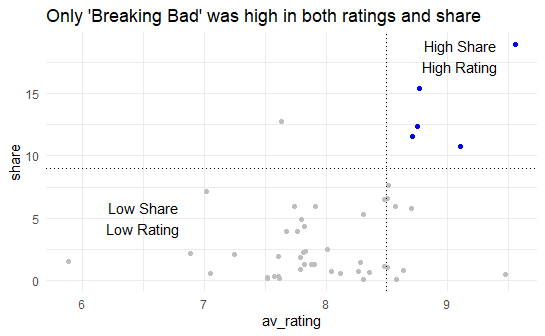
\includegraphics[width=1.82in,height=\textheight]{image/super-category.png}

::::

\section*{Social Media Preference
Example}\label{social-media-preference-example}
\addcontentsline{toc}{section}{Social Media Preference Example}

\markright{Social Media Preference Example}

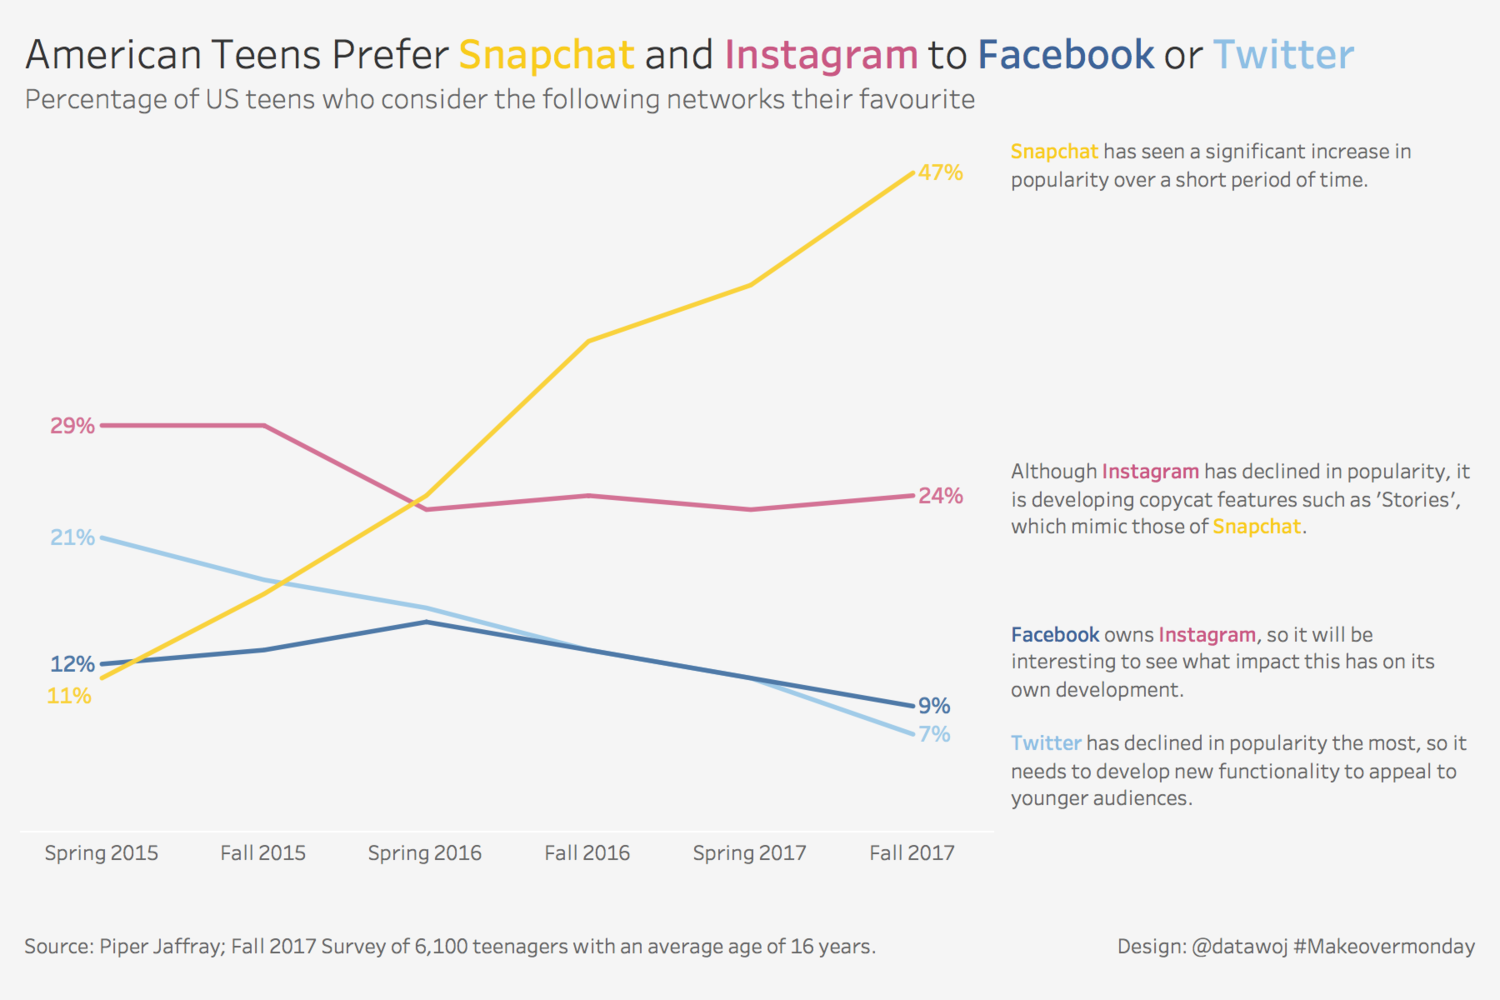
\includegraphics[width=5in,height=\textheight]{image/Colin.png}

https://datawoj.co.uk/visualising-data-on-which-social-media-network-us-teenagers-prefer/

\bookmarksetup{startatroot}

\chapter*{Part 3: Annotating}\label{part-3-annotating}
\addcontentsline{toc}{chapter}{Part 3: Annotating}

\markboth{Part 3: Annotating}{Part 3: Annotating}

\section*{Learning Objectives}\label{learning-objectives}
\addcontentsline{toc}{section}{Learning Objectives}

\markright{Learning Objectives}

\begin{itemize}
\tightlist
\item
  Learn about how annotations can help your viewer
\item
  Modify titles using \texttt{labs()}
\item
  Adding reference lines
\item
  Annotating directly onto the graph
\item
  Changing the scale
\end{itemize}

\section*{Before you move on,
discuss:}\label{before-you-move-on-discuss}
\addcontentsline{toc}{section}{Before you move on, discuss:}

\markright{Before you move on, discuss:}

What TV Show do you want to highlight with text? Why is it interesting
to you? Is there a trend you want to highlight?

\section*{Changing Titles}\label{changing-titles}
\addcontentsline{toc}{section}{Changing Titles}

\markright{Changing Titles}

There is a function called \texttt{labs()} that will let you change the
titles for a graph. Figure out where these titles are added to the graph
below.

\begin{Shaded}
\begin{Highlighting}[]
\NormalTok{my\_plot +}
\NormalTok{  labs(title = "Is it better to burn out than fade away?",}
\NormalTok{       x="Season Number", }
\NormalTok{       y="Average Rating")}
\end{Highlighting}
\end{Shaded}

Why is \texttt{labs()} not part of \texttt{theme()}? This is one
confusing thing about \texttt{ggplot2}. \texttt{theme()} is about the
\emph{appearance} (position, angle, font size) of an element, whereas
the \texttt{labs()} function actually provides the \emph{content}.

\section*{Adding a Reference Line}\label{adding-a-reference-line}
\addcontentsline{toc}{section}{Adding a Reference Line}

\markright{Adding a Reference Line}

Using \texttt{geom\_hline()} to show the average value across a time
period can provide a useful reference for viewers:

\begin{Shaded}
\begin{Highlighting}[]
\NormalTok{my\_plot + }
\NormalTok{  geom\_hline(yintercept = 7.8, lty=3)}
\end{Highlighting}
\end{Shaded}

We can add a vertical reference line instead using
\texttt{geom\_vline()} (note the argument, \texttt{xintercept} is
different than \texttt{geom\_hline()}):

\begin{Shaded}
\begin{Highlighting}[]
\NormalTok{my\_plot + }
\NormalTok{  geom\_vline(xintercept = 5, lty=3)}
\end{Highlighting}
\end{Shaded}

\section*{Adding text annotations}\label{adding-text-annotations}
\addcontentsline{toc}{section}{Adding text annotations}

\markright{Adding text annotations}

Adding text annotations directly to the graph can be extremely helpful,
especially if there are points of interest you want users to look at.
(For adding text information per data point, look at
\texttt{geom\_text()} and \texttt{geom\_repel()} from the
\texttt{ggrepel} package).

The first argument to \texttt{annotate()} is ``text''.

It takes \texttt{x} and \texttt{y} arguments to determine the position
of our annotation. These values are dependent on the scale - since we
have a numeric scale for both the \texttt{x} and \texttt{y} axes, we'll
use numbers to specify the position.

Our actual text goes in the \texttt{label} argument.

Run the code block below. Try adjusting the \texttt{y} argument for
\texttt{annotate()} to get the annotation more centered around the mean
reference line.

\begin{Shaded}
\begin{Highlighting}[]
\NormalTok{my\_plot + }
\NormalTok{  geom\_hline(yintercept = 7.8, lty=3) +}
\NormalTok{  annotate(geom="text", x = 2, y=10 , label="Mean Rating") }
\end{Highlighting}
\end{Shaded}

\section*{\texorpdfstring{One last thing: changing the numbers in the
ticks using
\texttt{scale\_x\_continuous()}}{One last thing: changing the numbers in the ticks using scale\_x\_continuous()}}\label{one-last-thing-changing-the-numbers-in-the-ticks-using-scale_x_continuous}
\addcontentsline{toc}{section}{One last thing: changing the numbers in
the ticks using \texttt{scale\_x\_continuous()}}

\markright{One last thing: changing the numbers in the ticks using
\texttt{scale\_x\_continuous()}}

One last thing that's been bugging me - the values of the ticks in the
\texttt{Season\ Number} axis. We can specify these numbers using the
\texttt{breaks} argument. Note that \texttt{c(1:10)} is a shortcut for
specifying \texttt{c(1,\ 2,\ 3,\ 4,\ 5,\ 6,\ 7,\ 8,\ 9,\ 10)}.

\begin{Shaded}
\begin{Highlighting}[]
\NormalTok{my\_plot + }
\NormalTok{  scale\_x\_continuous(breaks = c(1:10))}
\end{Highlighting}
\end{Shaded}

\section*{Part 3: Your Turn}\label{part-3-your-turn}
\addcontentsline{toc}{section}{Part 3: Your Turn}

\markright{Part 3: Your Turn}

Experiment with the following modifications to the graph. If you have
time, cut and paste the modifications you decided on in part 2 to your
graph.

If there's a show that you want to highlight, try adding an annotation
to highlight it. Or try adding an annotation at \texttt{Roseanne}'s
lowest rating!

\begin{Shaded}
\begin{Highlighting}[]
\NormalTok{\#put this in order}

\NormalTok{my\_plot + }
\NormalTok{    labs(title = "Is it better to burn out than fade away?",x="Season Number", y="Average Rating") + }
\NormalTok{  geom\_vline(xintercept = 5, lty=3) +}
\NormalTok{  annotate(geom="text", x = 7, y=8.5, label = "The Walking\textbackslash{}n Dead (brainzzz)") +}
\NormalTok{  scale\_x\_continuous(breaks = c(1:10))}
\end{Highlighting}
\end{Shaded}

\section*{For more information}\label{for-more-information}
\addcontentsline{toc}{section}{For more information}

\markright{For more information}

For more examples of how annotating can make figures more clear, please
check out Storytelling with Data: https://storytellingwithdata.com,
especially the linegraphs with annotations for examples:
http://www.storytellingwithdata.com/blog/2018/1/22/88-annotated-line-graphs

Making annotations first class citizens in data visualization:
https://medium.com/(\textbf{Elijah\_Meeks/making-annotations-first-class-citizens-in-data-visualization-21db6383d3fe?})

class: center, middle \# Part 4: Highlighting Data

\section*{Preattentive attributes}\label{preattentive-attributes}
\addcontentsline{toc}{section}{Preattentive attributes}

\markright{Preattentive attributes}

Color and contrast are known as \texttt{preattentive\ attributes}. Our
unconscious brain is aware of these kinds of attributes even before we
consciously process the content of a graph.

How many 3s are there in this image?

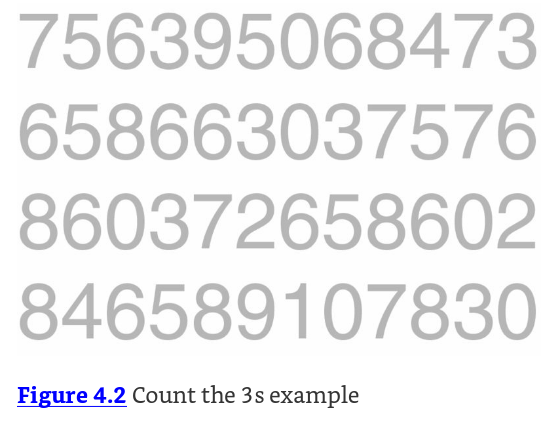
\includegraphics[width=1.86in,height=\textheight]{image/threes-grey.png}

\href{http://storytellingwithdata.com/}{Storytelling with Data}

\section*{How about now?}\label{how-about-now}
\addcontentsline{toc}{section}{How about now?}

\markright{How about now?}

You can use color and contrast to highlight aspects of the data. How
many 3s are there in this image now? Notice how much quicker you can
count them.

That's the power of preattentive attributes!

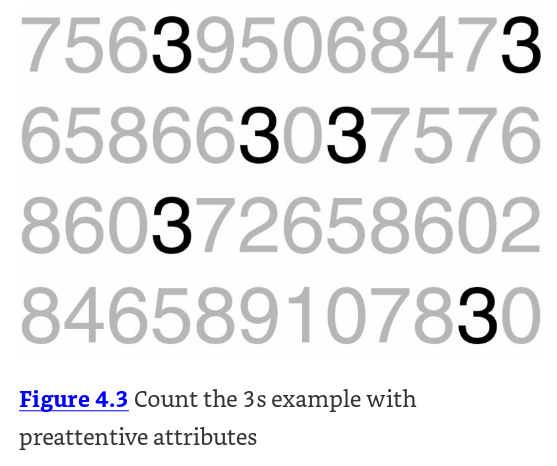
\includegraphics[width=1.86in,height=\textheight]{image/threes.png}

\href{http://storytellingwithdata.com/}{Storytelling with Data}

\section*{Best Practices for Using Color (Stephen
Few)}\label{best-practices-for-using-color-stephen-few}
\addcontentsline{toc}{section}{Best Practices for Using Color (Stephen
Few)}

\markright{Best Practices for Using Color (Stephen Few)}

\begin{itemize}
\tightlist
\item
  Use color only when needed to serve a particular communication goal
\item
  Use different colors only when they correspond to differences of
  meaning in the data.
\item
  Use soft, natural colors to display most information and bright and/or
  dark colors to highlight information that requires greater attention.
\end{itemize}

\href{http://www.perceptualedge.com/articles/visual_business_intelligence/rules_for_using_color.pdf}{Practical
Rules for Using Color}

\section*{Changing the base plot
(slightly)}\label{changing-the-base-plot-slightly}
\addcontentsline{toc}{section}{Changing the base plot (slightly)}

\markright{Changing the base plot (slightly)}

Remember our original plot mapped color to \texttt{title}. There's also
a variable called \texttt{status} in our data. \texttt{status} has two
different values: a tv show can be a \texttt{riser} (positive trend in
ratings), or be a \texttt{faller} (negative trend in ratings).

Let's modify the plot to use this variable to \texttt{color} our lines.
We'll save it as a different object, this time called
\texttt{my\_new\_plot}.

\begin{Shaded}
\begin{Highlighting}[]
\NormalTok{my\_new\_plot \textless{}{-} }
\NormalTok{  ggplot(tv\_shows) + }
\NormalTok{    aes(x = seasonNumber, }
\NormalTok{        y= av\_rating, }
\NormalTok{        group=title, }
\NormalTok{        color = status) +   \#changing \textasciigrave{}color\textasciigrave{} to map to \textasciigrave{}status\textasciigrave{} here}
\NormalTok{    geom\_line()}

\NormalTok{my\_new\_plot}
\end{Highlighting}
\end{Shaded}

\section*{Highlighting part of your
data}\label{highlighting-part-of-your-data}
\addcontentsline{toc}{section}{Highlighting part of your data}

\markright{Highlighting part of your data}

What if we only want to highlight one group in the data? In this case,
maybe we want to highlight the \emph{risers} in our dataset. If we color
them blue, and leave the others as \texttt{grey} we can immediately
highlight them as important and worth noticing in the context of the
other data.

We can actually manually color our traces by using
\texttt{scale\_color\_manual()}. This lets us manually map our values in
our variable (\texttt{riser} and \texttt{faller}) to colors:
(\texttt{blue} and \texttt{grey}).

\begin{Shaded}
\begin{Highlighting}[]
\NormalTok{my\_new\_plot + }
\NormalTok{  scale\_color\_manual(values=c("riser"="blue",}
\NormalTok{                              "faller"="grey")) +}
\NormalTok{  theme\_minimal()}
\end{Highlighting}
\end{Shaded}

If you've mapped a variable to \texttt{fill}, you'll have to use
\texttt{scale\_fill\_manual()} to map values to colors.

\subsection*{Try out mapping colors}\label{try-out-mapping-colors}
\addcontentsline{toc}{subsection}{Try out mapping colors}

Try using different colors to contrast the lines in the \texttt{values}
argument to \texttt{scale\_color\_manual()}. A small list of color names
in R can be found here:
https://www.r-graph-gallery.com/42-colors-names.html

\begin{Shaded}
\begin{Highlighting}[]
\NormalTok{library(tidyverse)}

\NormalTok{my\_new\_plot + }
\NormalTok{  scale\_color\_manual(values=c("riser"="blue", "faller"="grey"))}
\end{Highlighting}
\end{Shaded}

\section*{Put it all together!}\label{put-it-all-together}
\addcontentsline{toc}{section}{Put it all together!}

\markright{Put it all together!}

Cut and paste all your modifiers and make your final figure below!

\begin{Shaded}
\begin{Highlighting}[]
\NormalTok{my\_new\_plot +}
\NormalTok{  theme\_minimal()}
\end{Highlighting}
\end{Shaded}

\section*{Saving High Quality Plots}\label{saving-high-quality-plots}
\addcontentsline{toc}{section}{Saving High Quality Plots}

\markright{Saving High Quality Plots}

We can use \texttt{ggsave()} to save our plot. By default, it will save
the last plot we made.

\begin{Shaded}
\begin{Highlighting}[]
\NormalTok{ggsave("movieplot.pdf")}
\end{Highlighting}
\end{Shaded}

\section*{More Best Practices for
figures:}\label{more-best-practices-for-figures}
\addcontentsline{toc}{section}{More Best Practices for figures:}

\markright{More Best Practices for figures:}

Ten Simple Rules for Better Figures:
https://journals.plos.org/ploscompbiol/article?id=10.1371/journal.pcbi.1003833

\section*{More tips and tricks for using contrast and
color}\label{more-tips-and-tricks-for-using-contrast-and-color}
\addcontentsline{toc}{section}{More tips and tricks for using contrast
and color}

\markright{More tips and tricks for using contrast and color}

In \texttt{03-annotating}, we saw that we can specify the line type for
a particular graph. We can also specify line type as an aesthetic. Be
careful with line types - too many in a figure can obscure your point.

Shapes for points can also be helpful for highlighting particular data
points. Here's a useful reference.

More information here:
http://www.cookbook-r.com/Graphs/Shapes\_and\_line\_types/

\section*{Conclusions}\label{conclusions}
\addcontentsline{toc}{section}{Conclusions}

\markright{Conclusions}

Congrats! You're well on your way to learning how to make your figures
more accessible.

\section*{Putting it all Together}\label{putting-it-all-together}
\addcontentsline{toc}{section}{Putting it all Together}

\markright{Putting it all Together}

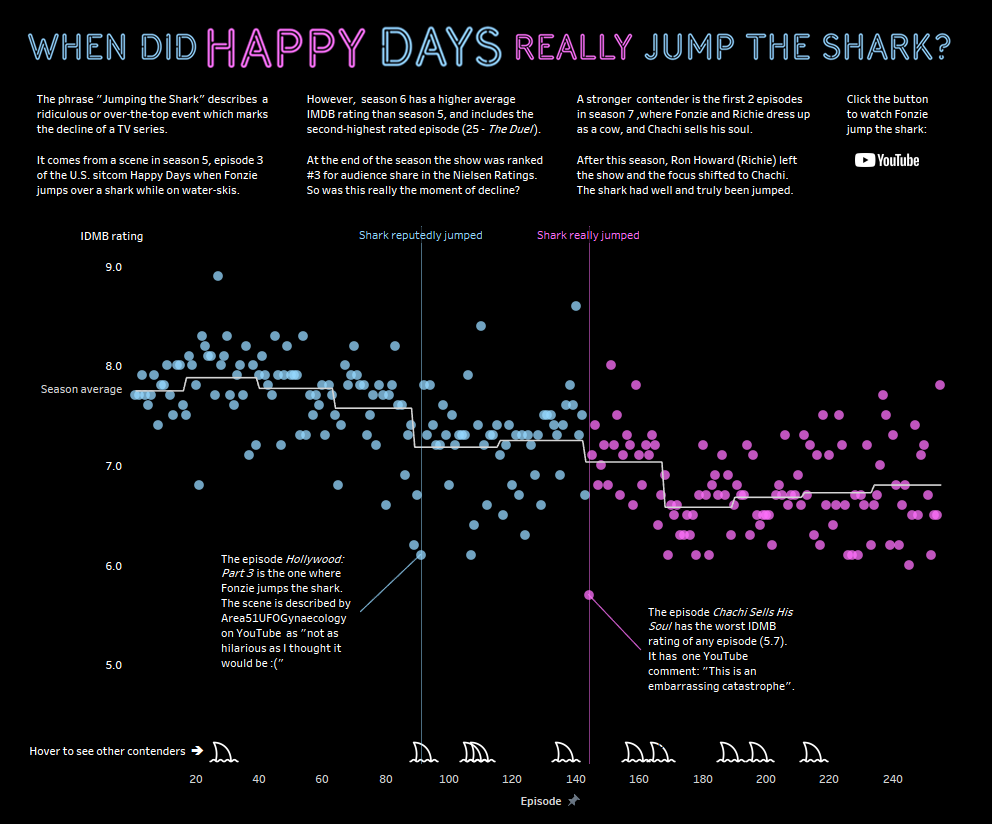
\includegraphics[width=3.31in,height=\textheight]{image/David_H.png}

\url{https://t.co/KSGQzaH0Mh}

\section*{Going Farther}\label{going-farther}
\addcontentsline{toc}{section}{Going Farther}

\markright{Going Farther}

\section*{\texorpdfstring{\texttt{ggplot2}
flipbook}{ggplot2 flipbook}}\label{ggplot2-flipbook}
\addcontentsline{toc}{section}{\texttt{ggplot2} flipbook}

\markright{\texttt{ggplot2} flipbook}

Good examples for styling your plots!

https://evamaerey.github.io/ggplot\_flipbook/ggplot\_flipbook\_xaringan.html

\begin{itemize}
\tightlist
\item
  \href{https://evamaerey.github.io/ggplot_flipbook/ggplot_flipbook_xaringan.html\#226}{Arctic
  Ice}
\item
  \href{https://evamaerey.github.io/ggplot_flipbook/ggplot_flipbook_xaringan.html\#302}{Flipping
  Seats}
\item
  \href{https://evamaerey.github.io/ggplot_flipbook/ggplot_flipbook_xaringan.html\#354}{Milk
  Cows}
\end{itemize}

\section*{Please fill out our survey!}\label{please-fill-out-our-survey}
\addcontentsline{toc}{section}{Please fill out our survey!}

\markright{Please fill out our survey!}

http://bit.ly/st\_survey

\section*{References}\label{references}
\addcontentsline{toc}{section}{References}

\markright{References}

\begin{itemize}
\tightlist
\item
  \href{http://www.storytellingwithdata.com/books}{Storytelling with
  Data}
\item
  \href{https://t.co/KSGQzaH0Mh}{Happy Days Jumping the Shark (Tableau
  Link)}
\item
  \href{https://evamaerey.github.io/ggplot_flipbook/ggplot_flipbook_xaringan.html}{\texttt{ggplot2}
  flipbook}
\item
  \href{https://alison.rbind.io/talk/2018-ohsu-sad-plot-better/}{Alison
  Hill: Take a Sad Plot and Make it Better}
\item
  Slides are done with xaringan/xaringanthemer
\end{itemize}

\section*{Keep in Touch}\label{keep-in-touch}
\addcontentsline{toc}{section}{Keep in Touch}

\markright{Keep in Touch}

\texttt{icon::fa("envelope")} tladera2 at fredhutch.org
\texttt{icon::fa("link")} https://laderast.github.io
\texttt{icon::fa("mastodon")} \href{https://vmst.io/@tladeras}{tladeras}

\bookmarksetup{startatroot}

\chapter{Setting up Our plot}\label{setting-up-our-plot}

Data4All

\hfill\break

\section{Motivation: Exploratory versus
Explanatory}\label{motivation-exploratory-versus-explanatory}

\textbf{Exploratory analysis}: - exploring and understanding the data,
conducting the analysis

\textbf{Explanatory analysis}: - explaining your findings from your
analysis in a coherent narrative that leads to a call to action

\section{Effective Visual
Communication}\label{effective-visual-communication}

Focus on three techniques:

\begin{itemize}
\tightlist
\item
  Decluttering your plot
\item
  Annotating your graph and data
\item
  Highlight data using Preattentive Attributes
\end{itemize}

\section{Paper Doll Approach}\label{paper-doll-approach}

\begin{itemize}
\tightlist
\item
  We're going to take a basic plot and dress it up
\item
  Modify its appearance to make our point more understandable and
  immediate
\end{itemize}

\includegraphics{image/giphy.gif}

\section{Assigning our plot so we can reuse it (3
min).}\label{assigning-our-plot-so-we-can-reuse-it-3-min.}

Let's save our plot into an R object called a ggplot. We'll use the
\texttt{\textless{}-} (left arrow) to assign it to the variable called
\texttt{my\_plot}:

\begin{Shaded}
\begin{Highlighting}[]
\NormalTok{\#| exercise: ex1}
\NormalTok{my\_plot \textless{}{-} }
\NormalTok{  ggplot(tv\_shows) +}
\NormalTok{  aes(x = seasonNumber, }
\NormalTok{      y = av\_rating, }
\NormalTok{      group = title, }
\NormalTok{      color = title) + }
\NormalTok{  geom\_line()}
\end{Highlighting}
\end{Shaded}

\section{\texorpdfstring{Dressing up
\texttt{my\_plot}}{Dressing up my\_plot}}\label{dressing-up-my_plot}

Now, when we want to modify our plot, we can use \texttt{my\_plot}. More
on this in the next notebook. We're basically going to add commands to
modify our plot. I like to think of it as a \texttt{paper\ doll}
approach: we are dressing our plot in different clothes.

\begin{Shaded}
\begin{Highlighting}[]
\NormalTok{my\_plot}
\end{Highlighting}
\end{Shaded}

\bookmarksetup{startatroot}

\chapter{Decluttering Plots}\label{decluttering-plots}

\bookmarksetup{startatroot}

\chapter{Part 2: Declutter your
graph}\label{part-2-declutter-your-graph}

\section{Why do we need to declutter our
graphs?}\label{why-do-we-need-to-declutter-our-graphs}

\begin{itemize}
\tightlist
\item
  Reduce cognitive load (help tired and cranky viewers)
\item
  Viewer can focus on what matters
\item
  Not all information is useful for your viewer
\end{itemize}

\section{Example: London Subway
Diagram}\label{example-london-subway-diagram}

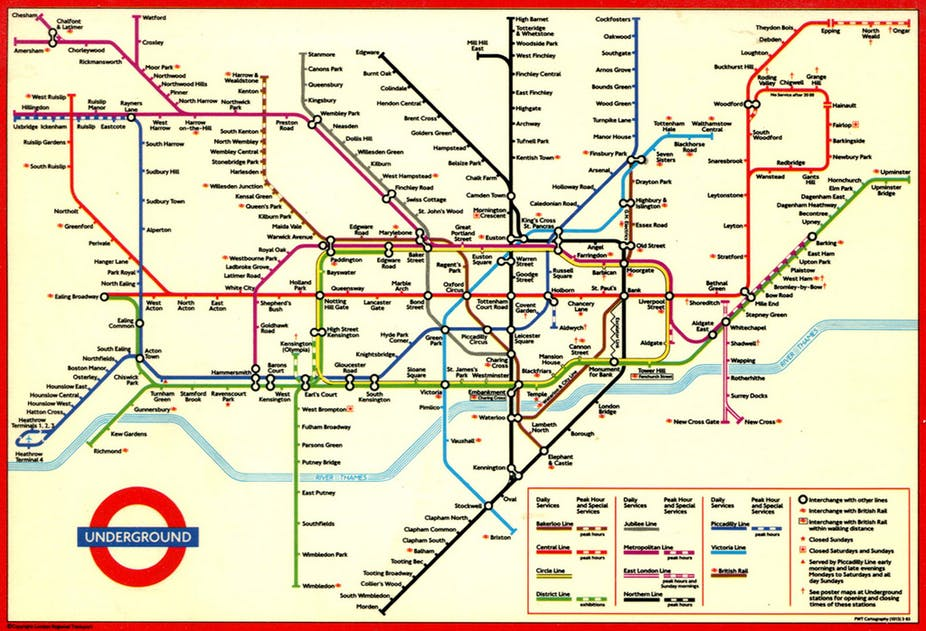
\includegraphics{image/london-underground.jpg}

\begin{itemize}
\tightlist
\item
  Triumph of minimal design
\item
  Removes geography
\item
  Emphasizes: what lines to I take to get from A to B?
\end{itemize}

\url{http://theconversation.com/sublime-design-the-london-underground-map-26240}

\section{Cognitive Load}\label{cognitive-load}

\begin{itemize}
\tightlist
\item
  Think of your audience:

  \begin{itemize}
  \tightlist
  \item
    Tired and cranky and want you to get to the point!
  \item
    Short term memory 5 +/- 2 things at once
  \end{itemize}
\item
  Remove elements that distract from your message

  \begin{itemize}
  \tightlist
  \item
    Shadows, 3D Effects
  \item
    Legends/too many colors
  \item
    Axis Titles (sometimes)
  \end{itemize}
\end{itemize}

\section{Ask Yourself}\label{ask-yourself}

\begin{itemize}
\tightlist
\item
  Does this element support
  \href{http://www.storytellingwithdata.com/blog/2017/3/29/declutter-this-graph}{the
  point I want to make about the data?}
\end{itemize}

\begin{Shaded}
\begin{Highlighting}[]
\NormalTok{\#| echo: false}
\NormalTok{knitr::include\_graphics("image/before{-}after.png")}
\end{Highlighting}
\end{Shaded}

\section{Theming}\label{theming}

The neat thing about \texttt{ggplot2} is that you can modify the plot
code by adding \emph{modifiers} with the \texttt{+} (plus) sign.

We're going to take a ``paper doll'' approach to our plot to modifying
it - each \emph{modifier} can be thought of as a set of ``clothes'' that
we dress our plot in.

\section{Removing Stuff}\label{removing-stuff}

The defaults for the plot are decent, but have some distracting
elements. We can declutter our plot by removing some of these
distracting elements.

Before you move on, discuss on slack:

\begin{enumerate}
\def\labelenumi{\arabic{enumi})}
\tightlist
\item
  What parts of the plot are distracting from your message about tv
  shows that are \texttt{risers}?
\end{enumerate}

\section{One note}\label{one-note}

In each section, we're trying different types of modification, so
they're not cumulative. However, you can cut and paste the modifications
together in the end to have your final customized plot.

\section{Intelligent Defaults: Using Built in
Themes}\label{intelligent-defaults-using-built-in-themes}

A lot of the simplification can come from built in themes. Themes are
like a full wardrobe for our paper dolls, specifying lots of different
details.

Adding \texttt{theme\_minimal()} will remove a lot of the background
elements. Try it out and compare it with the above plot.

Built in themes let you be more efficient in paring elements down, but
you will often find that you need to customize them. That's what we'll
look at next.

\begin{Shaded}
\begin{Highlighting}[]
\NormalTok{my\_plot + theme\_minimal()}
\end{Highlighting}
\end{Shaded}

\section{\texorpdfstring{Removing elements using
\texttt{theme()}}{Removing elements using theme()}}\label{removing-elements-using-theme}

We can customize our plot even further by adding a \texttt{theme()}
function to the end of our plot. We'll use this to remove individual
elements from the plot.

Note: If we change any theme attributes after calling
\texttt{theme\_minimal()}, it will basically \emph{overwrite} the
previous built-in theme. This means that order is important, so keep
that in mind!

\texttt{theme()} looks very intimidating, because it has lots of
different arguments. We'll only look at a few of these:

\begin{itemize}
\tightlist
\item
  \texttt{axis.title}, \texttt{axis.title.x} and \texttt{axis.title.y}
  (The labels for the axes)
\item
  \texttt{panel.grid} (grid lines)
\item
  \texttt{legend.position} (Placing the legend, including removing it)
\end{itemize}

How will we remove these elements? For most of them, we will specify an
element called \texttt{element\_blank()} to these arguments. What is
this? Think of it as a special placeholder that says we don't want to
see this element.

\section{Remove some Text}\label{remove-some-text}

Let's try simplifying our plot by removing the x-axis text. By context,
the label \texttt{seasonNumber} isn't that helpful.

\begin{Shaded}
\begin{Highlighting}[]
\NormalTok{my\_plot + }
\NormalTok{  theme(axis.title.x = element\_blank())}
\end{Highlighting}
\end{Shaded}

\section{Remove the Gridlines}\label{remove-the-gridlines}

Try removing the gridlines. Is that helpful or not?

\begin{Shaded}
\begin{Highlighting}[]
\NormalTok{my\_plot + }
\NormalTok{  theme(panel.grid = element\_blank())}
\end{Highlighting}
\end{Shaded}

\section{Remove the Legend}\label{remove-the-legend}

Sometimes, to remove some items, like the legend, you have to specify it
not as \texttt{element\_blank}, but as ``none''. Try removing the
legend.

Hmm, it is more simplified, but we have lost all the information about
the categories! We can add that information back with the use of color
in section 3.

\begin{Shaded}
\begin{Highlighting}[]
\NormalTok{my\_plot + }
\NormalTok{  theme(legend.position = "none")}
\end{Highlighting}
\end{Shaded}

\section{Your turn}\label{your-turn}

Play with different combinations of these different \texttt{theme()}
statements to customize your plot. If you want to remove a line, you can
put a \texttt{\#} in front of that line. That will make it a comment and
that line of code won't run.

\begin{Shaded}
\begin{Highlighting}[]
\NormalTok{my\_plot +}
\NormalTok{  theme\_minimal() + }
\NormalTok{  \#theme(axis.title.x = element\_blank()) + }
\NormalTok{  theme(panel.grid = element\_blank()) + }
\NormalTok{  theme(legend.position = "none")}
\end{Highlighting}
\end{Shaded}

\section{For more information}\label{for-more-information-1}

Take a look at the ggthemes gallery for other pre-made themes that can
help you declutter your plot.

https://www.datanovia.com/en/blog/ggplot-themes-gallery/

Look at the documentation for \texttt{theme()} to understand how to
customize different elements. Each element maps to four different
elements:

\texttt{element\_blank()} - we've seen this. \texttt{element\_text()} -
anything that's text (such as labels - this is where you can specify
arguments like \texttt{angle},\texttt{size}) \texttt{element\_rect()} -
anything that's a rectangle (such as the panel) \texttt{element\_line()}
- anything that's a line (such as axes and grid lines)




\end{document}
